%02.11.2018
\section{Funktionen und Abbildungen}
\subsection{Funktion als Abbildung}
\begin{defi}
	Eine Funktion (oder Abbildung) von einer Menge $A$ in eine Menge $B$ ordnet jedem Element $a\in A$ ein eindeutiges Element $b \in B$ zu.\\
	Wir schreiben:
	\begin{equation*}
		f: A \rightarrow B, a \mapsto f(a)\quad(=b)
	\end{equation*}	
	$A$: Definitionsbereich\\
	$B:$ Zielbereich (Target(space))\\
	z.B. $f: \mathbb{R} \rightarrow \mathbb{R}, x \mapsto x^2$\\
	Die Abbildung $f: A \rightarrow B$ ist\\
	\begin{tabular}{r|l}
		injektiv&aus $f(a) = f(a') \; a, a' \in A$, folgt $a=a'$\\
		surjektiv&$\forall b\in B \exists a\in A: b=f(a)$\\
		bijektiv&sie ist injektiv und surjektiv
	\end{tabular}
\end{defi}
\begin{bem}
	$f: A\rightarrow B$ injektiv $\Leftrightarrow a, a'\in A, a \neq a' \Rightarrow f(a) \neq f(a')$
\end{bem}
$f: A\rightarrow B$ ist bijektiv $\Rightarrow \forall b\in B \exists ! a\in A: f(a) = b$.\\
Definiere, wenn bijektiv $f^{-1}: B\rightarrow A, b\mapsto a, a\in A: f(a) = b$\\(inverse Funktion).\\
Ist $f: A\rightarrow B$ nicht bijektiv. (Verallgemeinerte Inverse)\\
$f^{-1}: P(B)\rightarrow P(A), M \mapsto\{a\in A|f(a)\in M\}$\\
Verkettung:\\
gegeben: $f:A\rightarrow B, g: B\rightarrow C$\\
$g\circ f: A\rightarrow C\qquad g\circ f(a):= g(f(a))$.\\
$A\overset{f}{\rightarrow} B \overset{g}{\rightarrow}C$\\
$f: A\rightarrow B$ ist bijektiv $\Rightarrow f^{-1}\circ f = \operatorname{id}_A, f\circ f^{-1} = \operatorname{id}_B$\\
$\operatorname{id}_A: A\rightarrow A, a\mapsto a.$
\subsection{Abbildungen als Graph}
\begin{defi}
	Seien $A,B$ Mengen. Dann ist $(a,b)$ ein sog. Tupel.\\
	in der Mengenlehre: $(a,b) := \{\{a\}, \{a,b\}\}$.
\end{defi}
Beachte: Reihenfolge ist wichtig! im Allg. $(a,b)\neq (b,a)$\\
Menge $A\times B := \{(a,b)|a\in A, b\in B\}$\\
heißt kartesisches Produkt (von $A$ und $B$)\\
z.B. $\mathbb{R}\times\mathbb{R}$\\
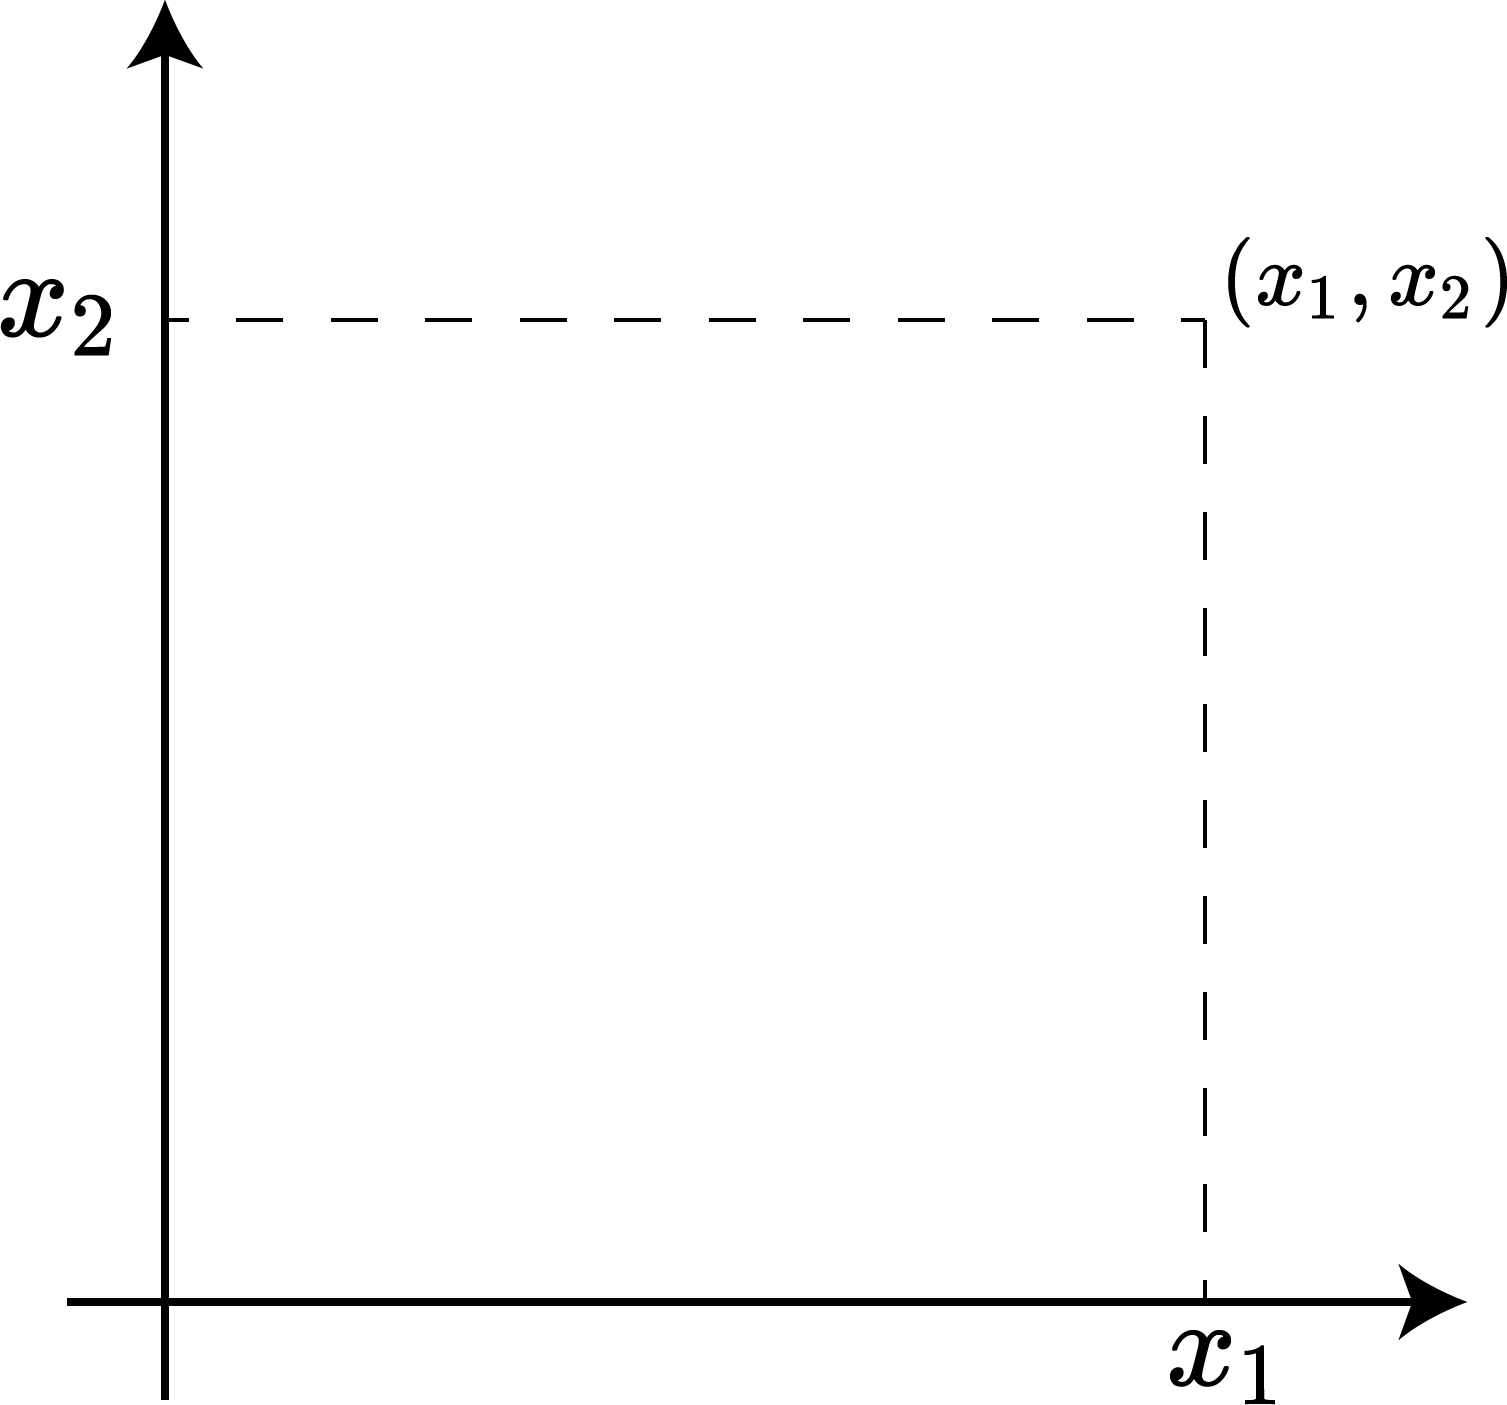
\includegraphics[width=0.3\textwidth]{images/img03.png}\\
\textbf{2. Abbildungen Projektionen}\\
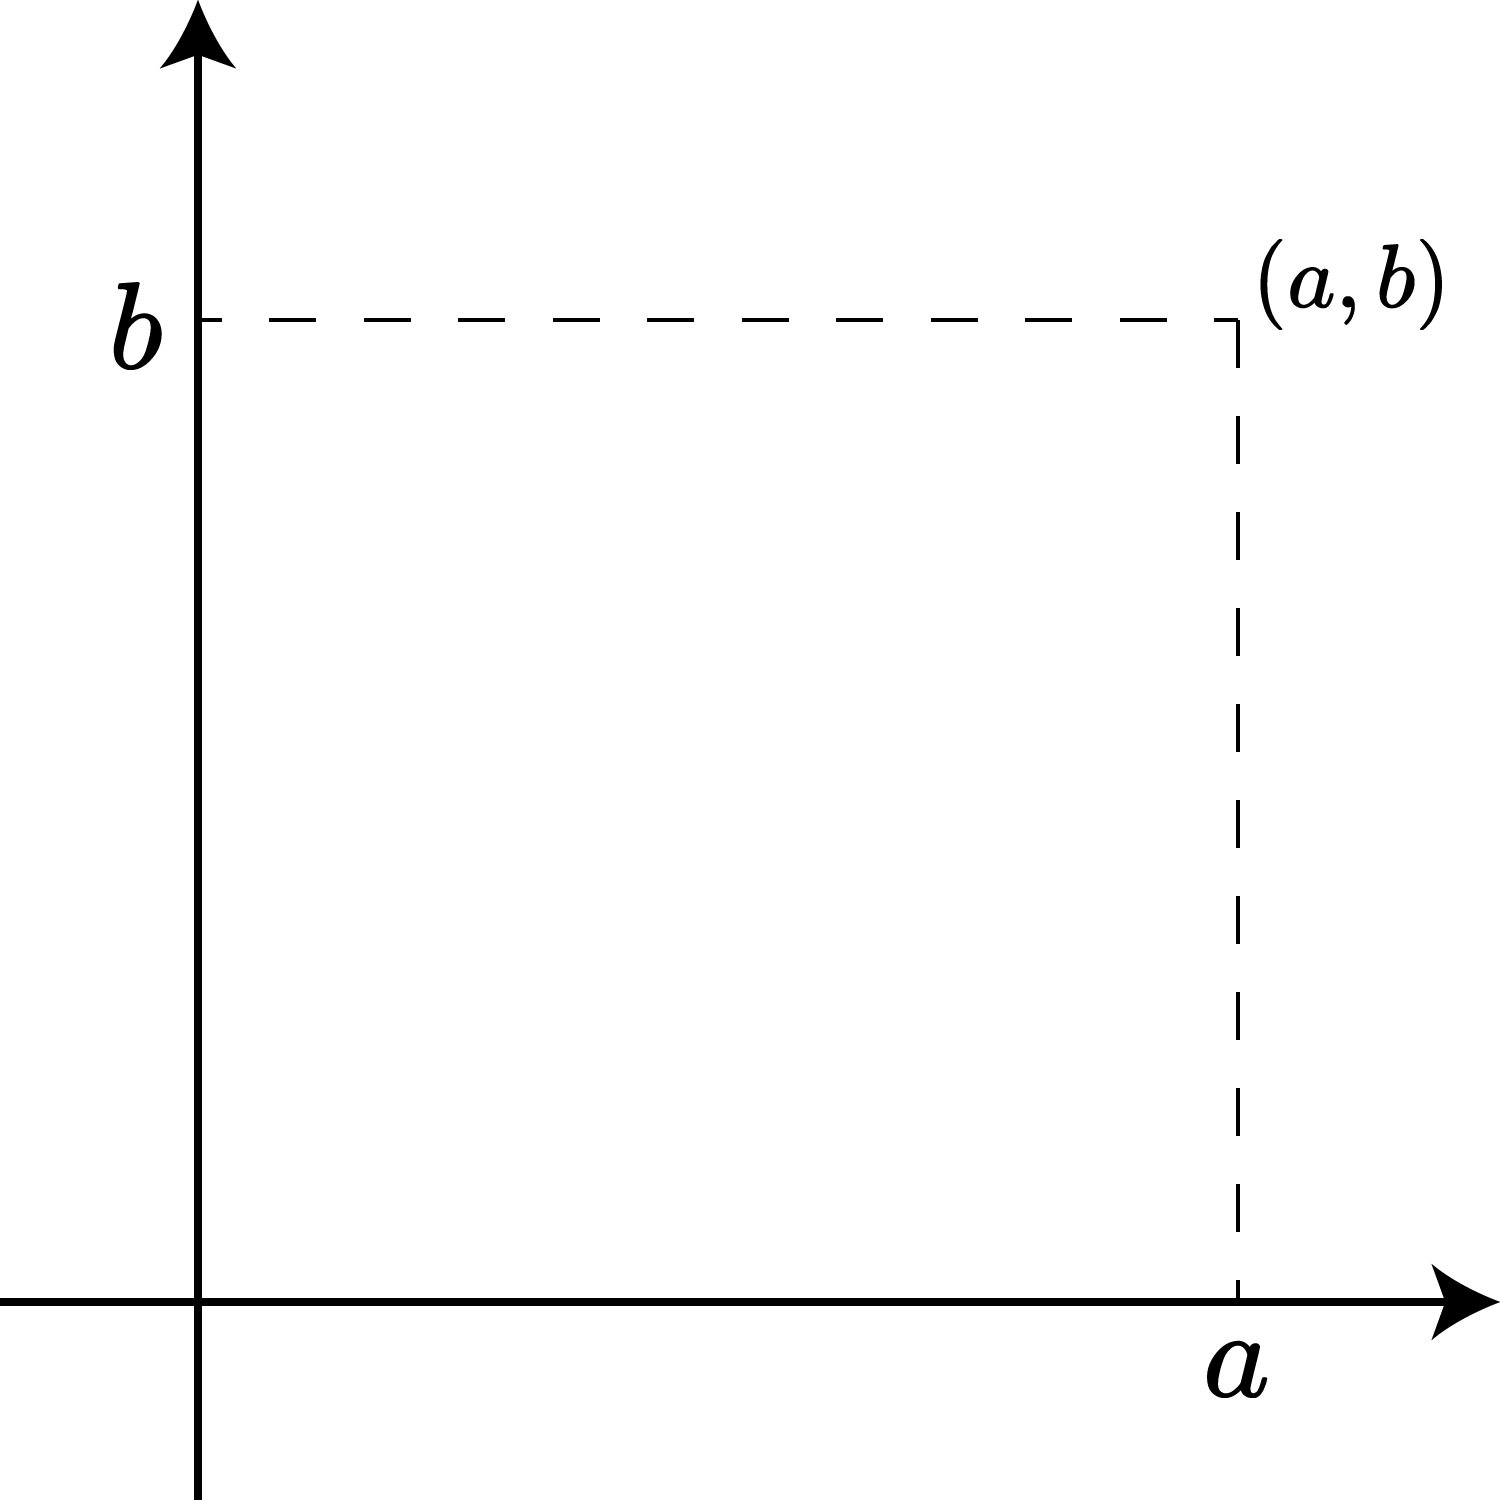
\includegraphics[width=0.3\textwidth]{images/img04.png}\\
$\Pi_1 = \Pi_A : A\times B \rightarrow A, (a,b)\mapsto a$ (Projektion auf 1. Koordinate)\\
$\Pi_2 = \Pi_B : A\times B \rightarrow B, (a,b) \mapsto b$ (Projektion auf 2. Koordinate)\\
$\Pi_A(a,b) = a$\\
$\Pi_B(a,b) = b$\\
$n$-Tupel: Mengen $A_1,\dots ,A_n, n\in \mathbb{N}.$\\
$A_1\times A_2$ wie vorhin\\
$A_1\times\dots\times A_{n+1} := (A_1\times\dots\times A_n)\times A_{n+1}, n\in \mathbb{N}$ (induktiv)\\
Beobachtung:\\
$(A\times B)\times C = A\times (B\times C) + \{(a,b,c)|a\in A, b\in B, c\in C\} = ((a,b),c) = (a,(b,c))$\\
Genauer: $\exists$ Bijektion $\Phi : (A\times B) \times C \rightarrow A\times (B\times C)$

\begin{defi}[Graph einer Abbildung]
	Geg: $f: A \rightarrow B$ Funktion\\
	$\Gamma := \Gamma_f := \{(a,b) \in A\times B : b = f(a)\} \subset A\times B$\\
	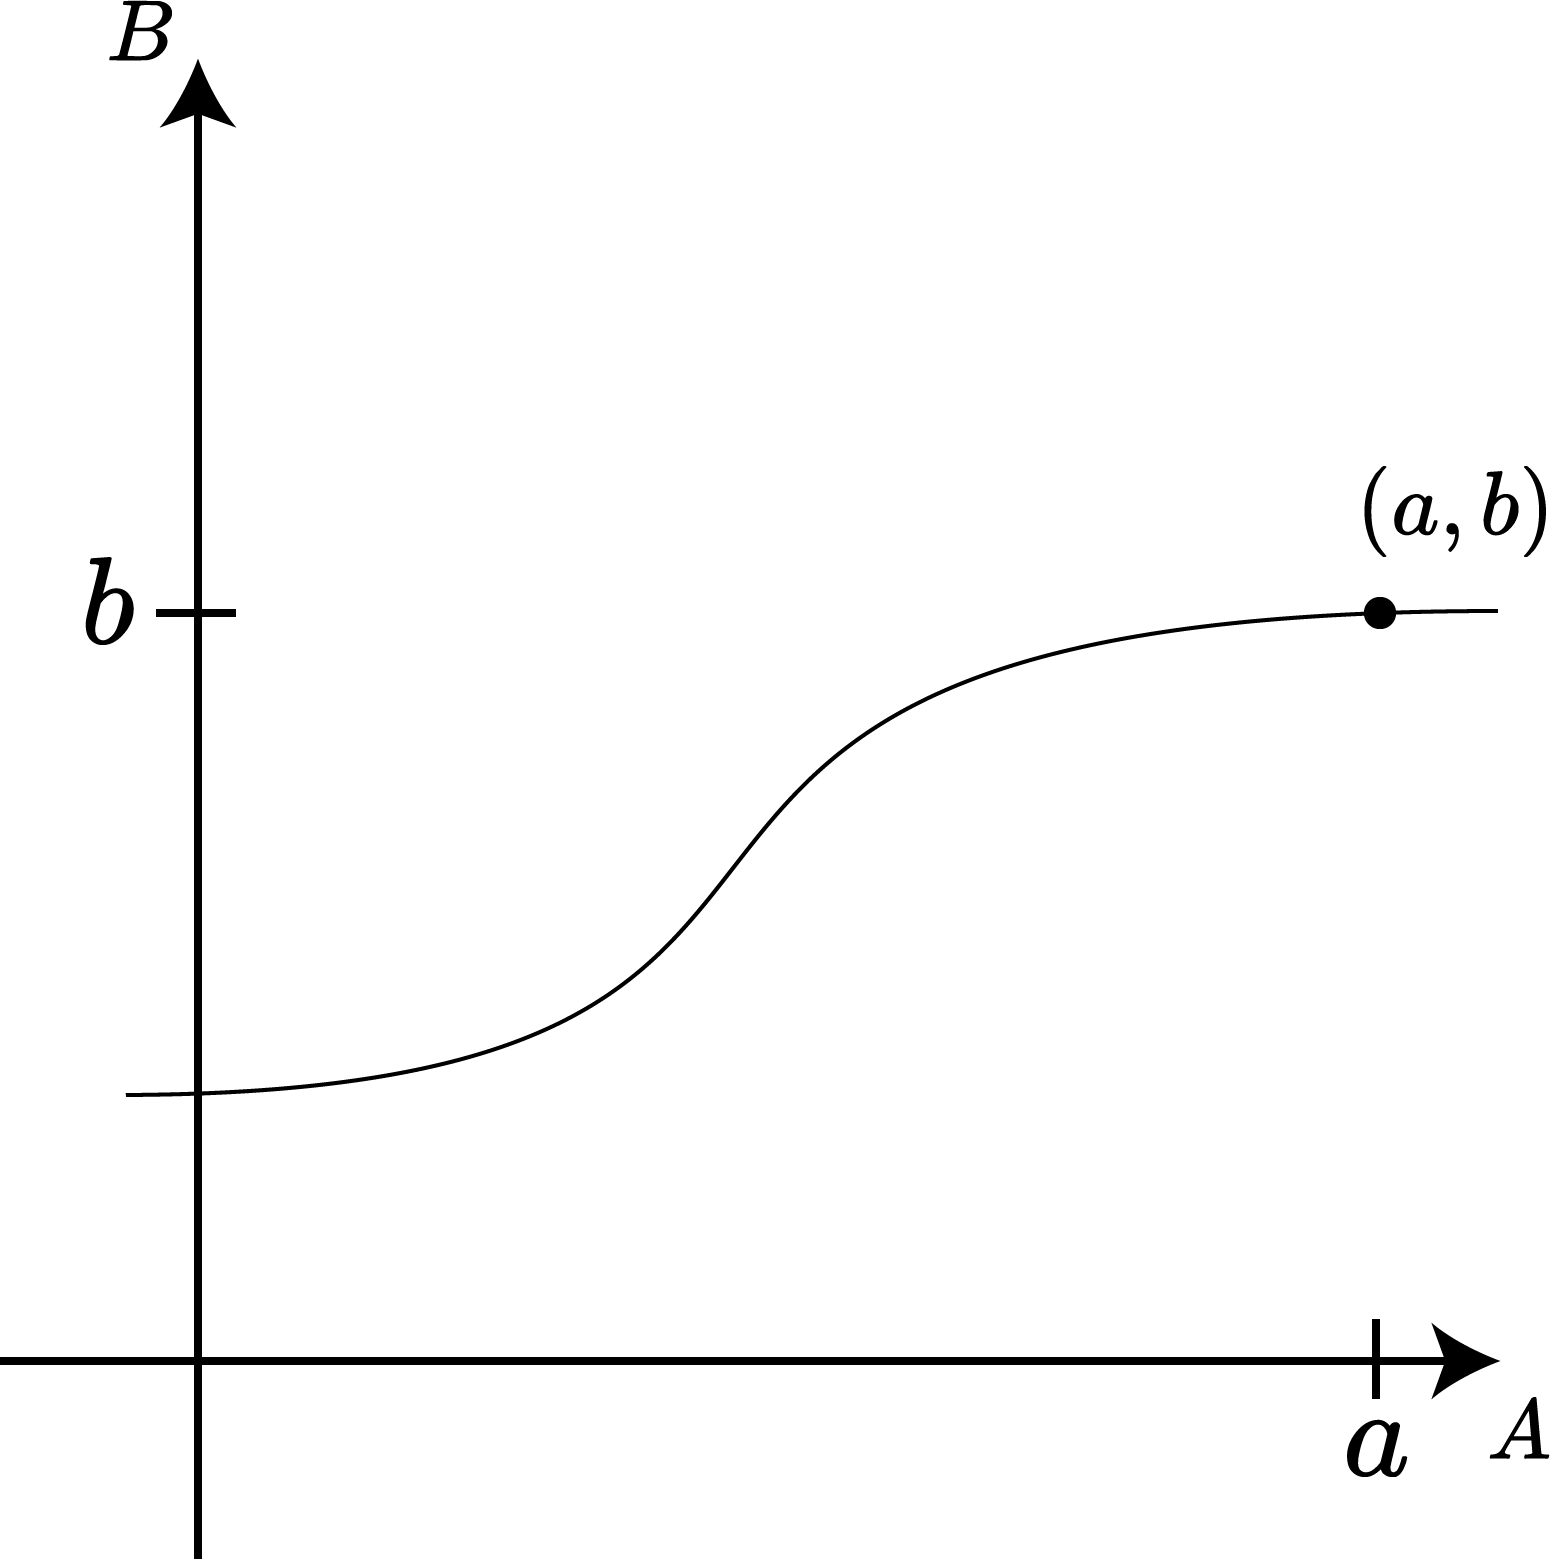
\includegraphics[width=0.3\textwidth]{images/img05.png}
	\quad
	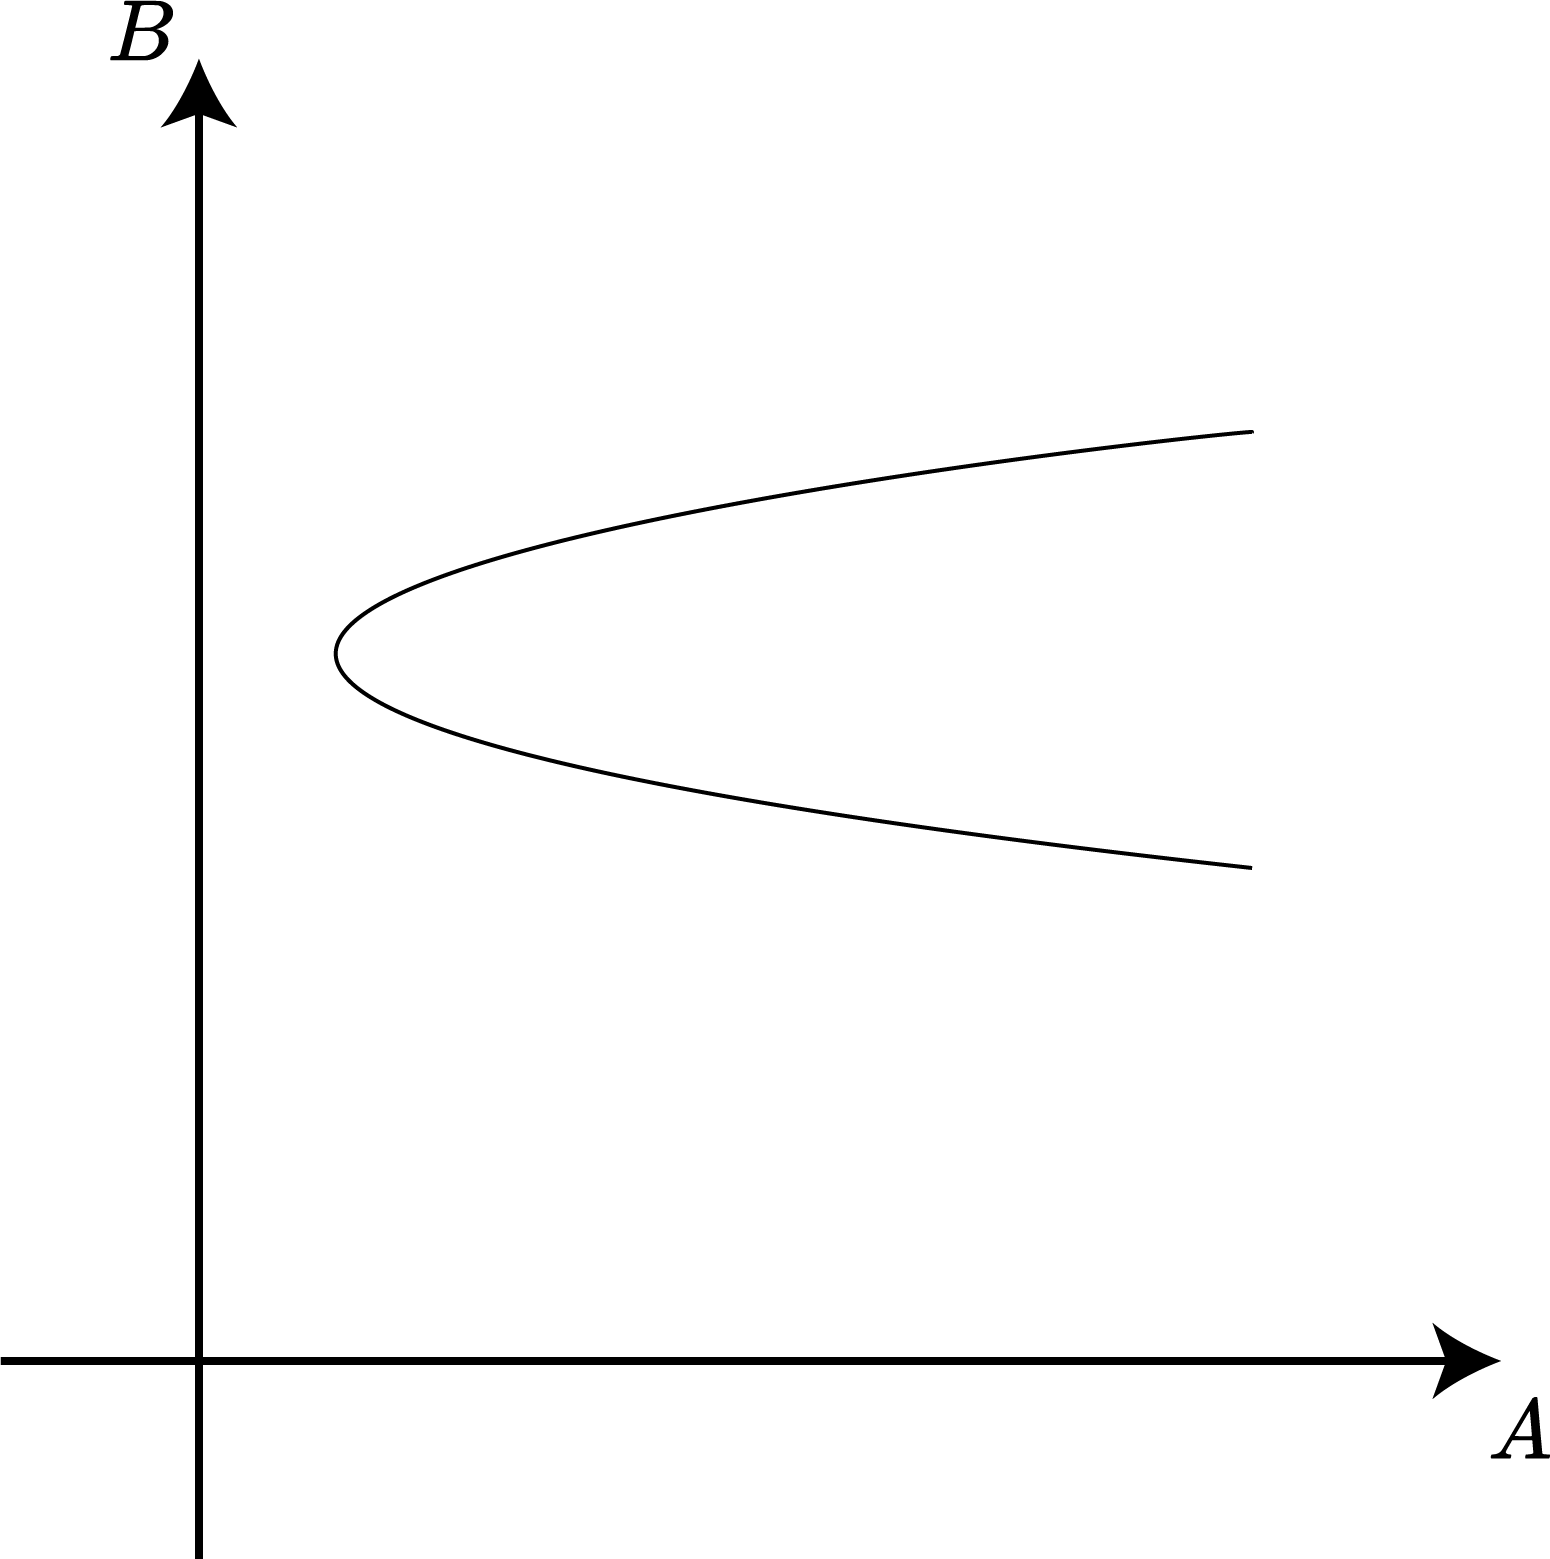
\includegraphics[width=0.3\textwidth]{images/img06.png}\\
	$P\subset A\times B$ ist der Graph einer Funktion genau dann, wenn aus $(a_1,b_1), (a_2,b_2) \in \Gamma$ folgt $b_1 = b_2$. (und $\forall a\in A \exists b\in B:(a,b)\in\Gamma$)
\end{defi}
\begin{satz}
	$\Gamma \subset A\times B$ ist genau dann Graph einer Abbildung $f: A\rightarrow B$, wenn die Projektion $\Pi_A \vert_\Gamma : \Gamma \rightarrow A$ bijektiv ist.\\
	Notation: $g: D \rightarrow E, X\subset D$\\
	$g\vert_X: X\rightarrow E, x\mapsto g(x)$\\
\end{satz}
\begin{bew}
	Sei $\Gamma = \Gamma_f$ mit $f: A\rightarrow B$ Funktion\\
	$\overset{(a,b)\in \Gamma_f \Leftrightarrow b = f(a)}{\Rightarrow} \forall a\in A$ existiert genau ein $b\in B$ mit $f(a) = b$.\\
	$\Rightarrow \Pi_A \vert_\Gamma$ ist bijektiv.\\
	Umgekehrt: Sei $\Pi_A \vert_\Gamma \rightarrow A$ bijektiv.\\
	D.h. ist $(a_j, b_j) \in \Gamma, j \in\{1,2\}$\\
	und $\Pi_A(a_1, b_1) = \Pi_A(a_2, b_2) \Rightarrow (a_1, b_1) = (a_2, b_2)$\\
	$\Leftrightarrow a_1 = a_2, b_1 = b_2$\\
	$\Rightarrow$ zu $a\in A \exists ! b\in B, (a,b) \in \Gamma$.\\
	Da $b=\Pi_B(a,b) = \Pi_B((\Pi_A\vert_\Gamma)^{-1}(a))$\\
	Definiere $f:= \Pi_B \circ (\Pi_A\vert_\Gamma)^{-1}:A\rightarrow B$ ist Funktion\\
	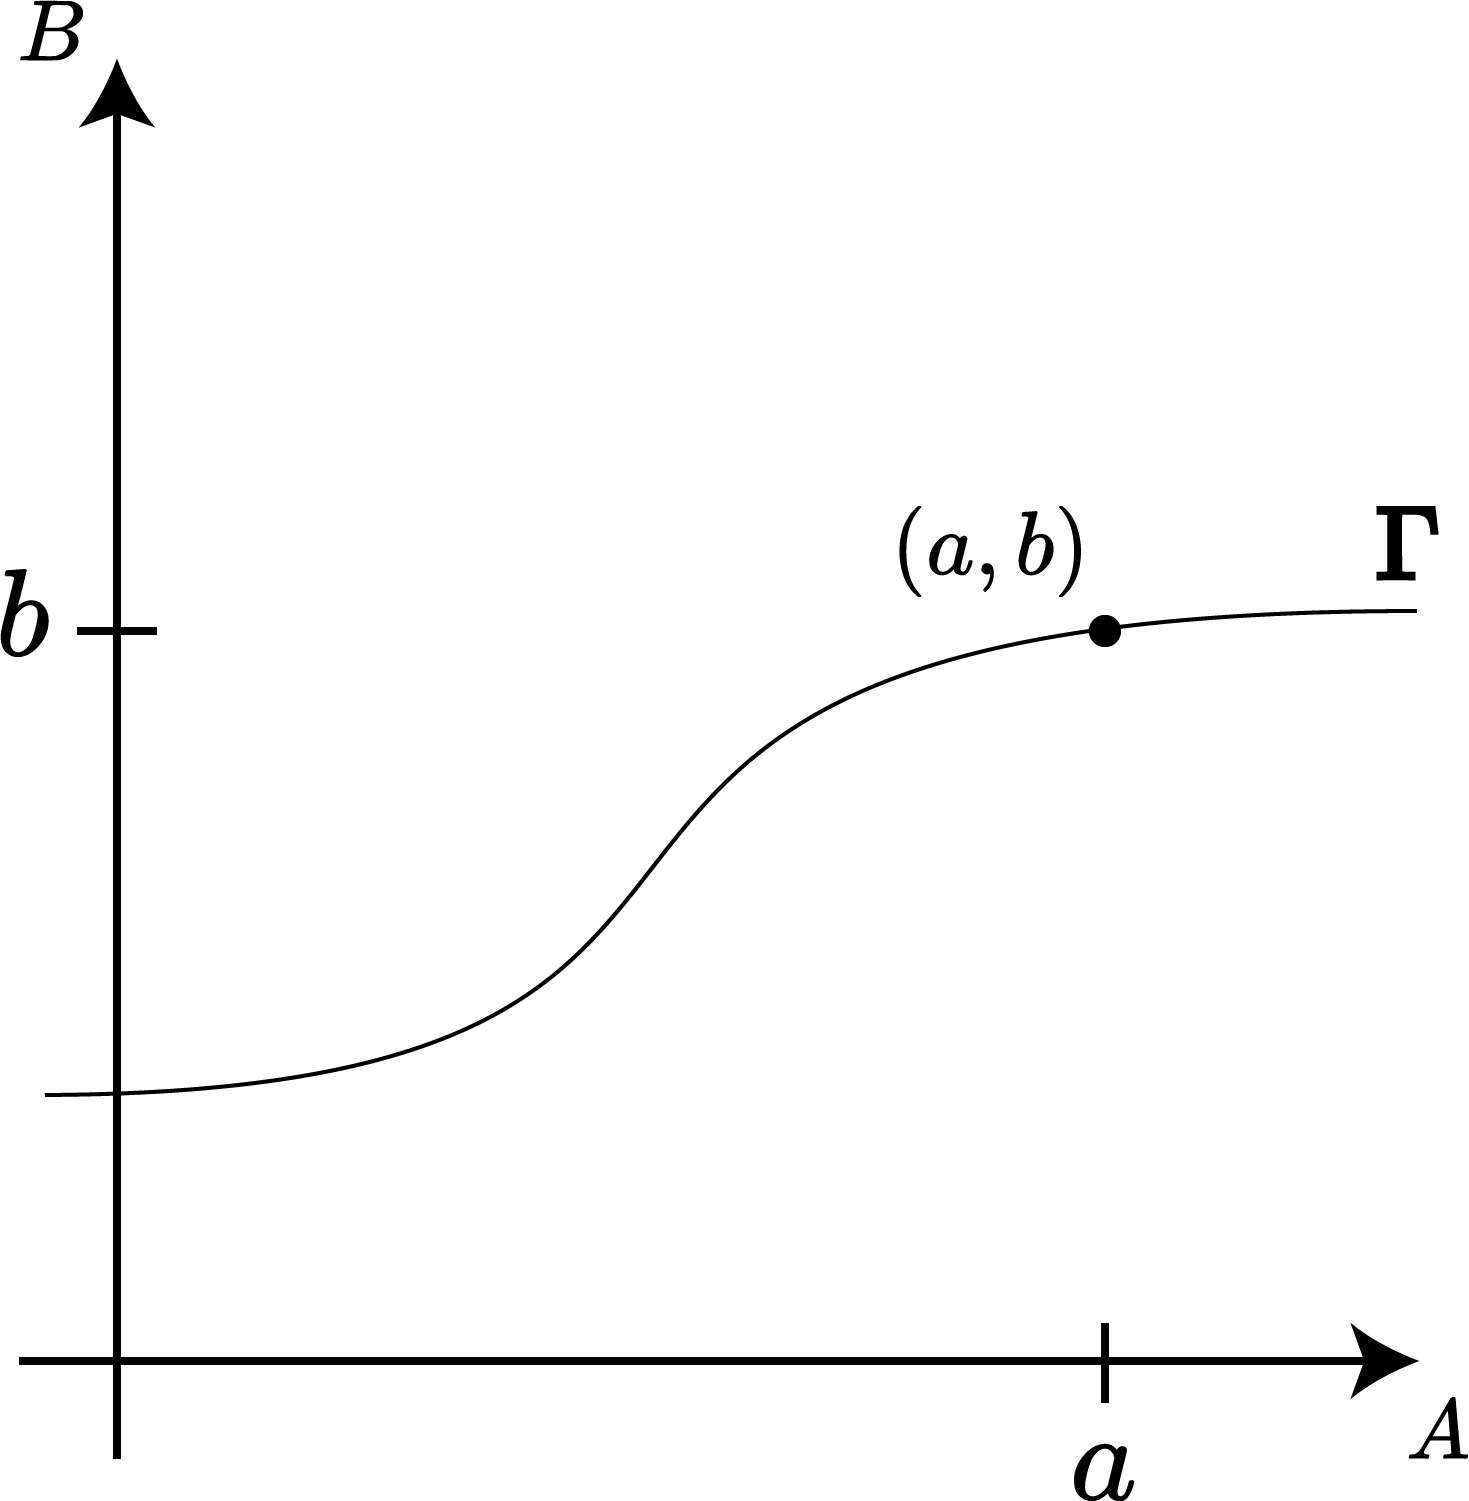
\includegraphics[width=0.3\textwidth]{images/img07.png}\\
	nachrechnen $\Gamma = \Gamma_f$
\end{bew}
\begin{bem}
	In Satz 3 gilt $f = \Pi_B \circ (\Pi_A\vert_\Gamma)^{-1}$ %ENTSPRICHT 4.2
\end{bem}
\begin{bsp}
	Ist $f: A\rightarrow B$ bijektiv\\
	$b=f(a),\quad f^{-1}(b)=a$\\
	Dann gilt: $\Gamma_f^{-1} = \{(b, f^{-1}(b)) | b\in B\}\\
	= \{(f(a),a):a\in A\} = S(\Gamma_f), S: A\times B \rightarrow B\times A$ (swap), $(a,b)\mapsto(b,a)$.\\
	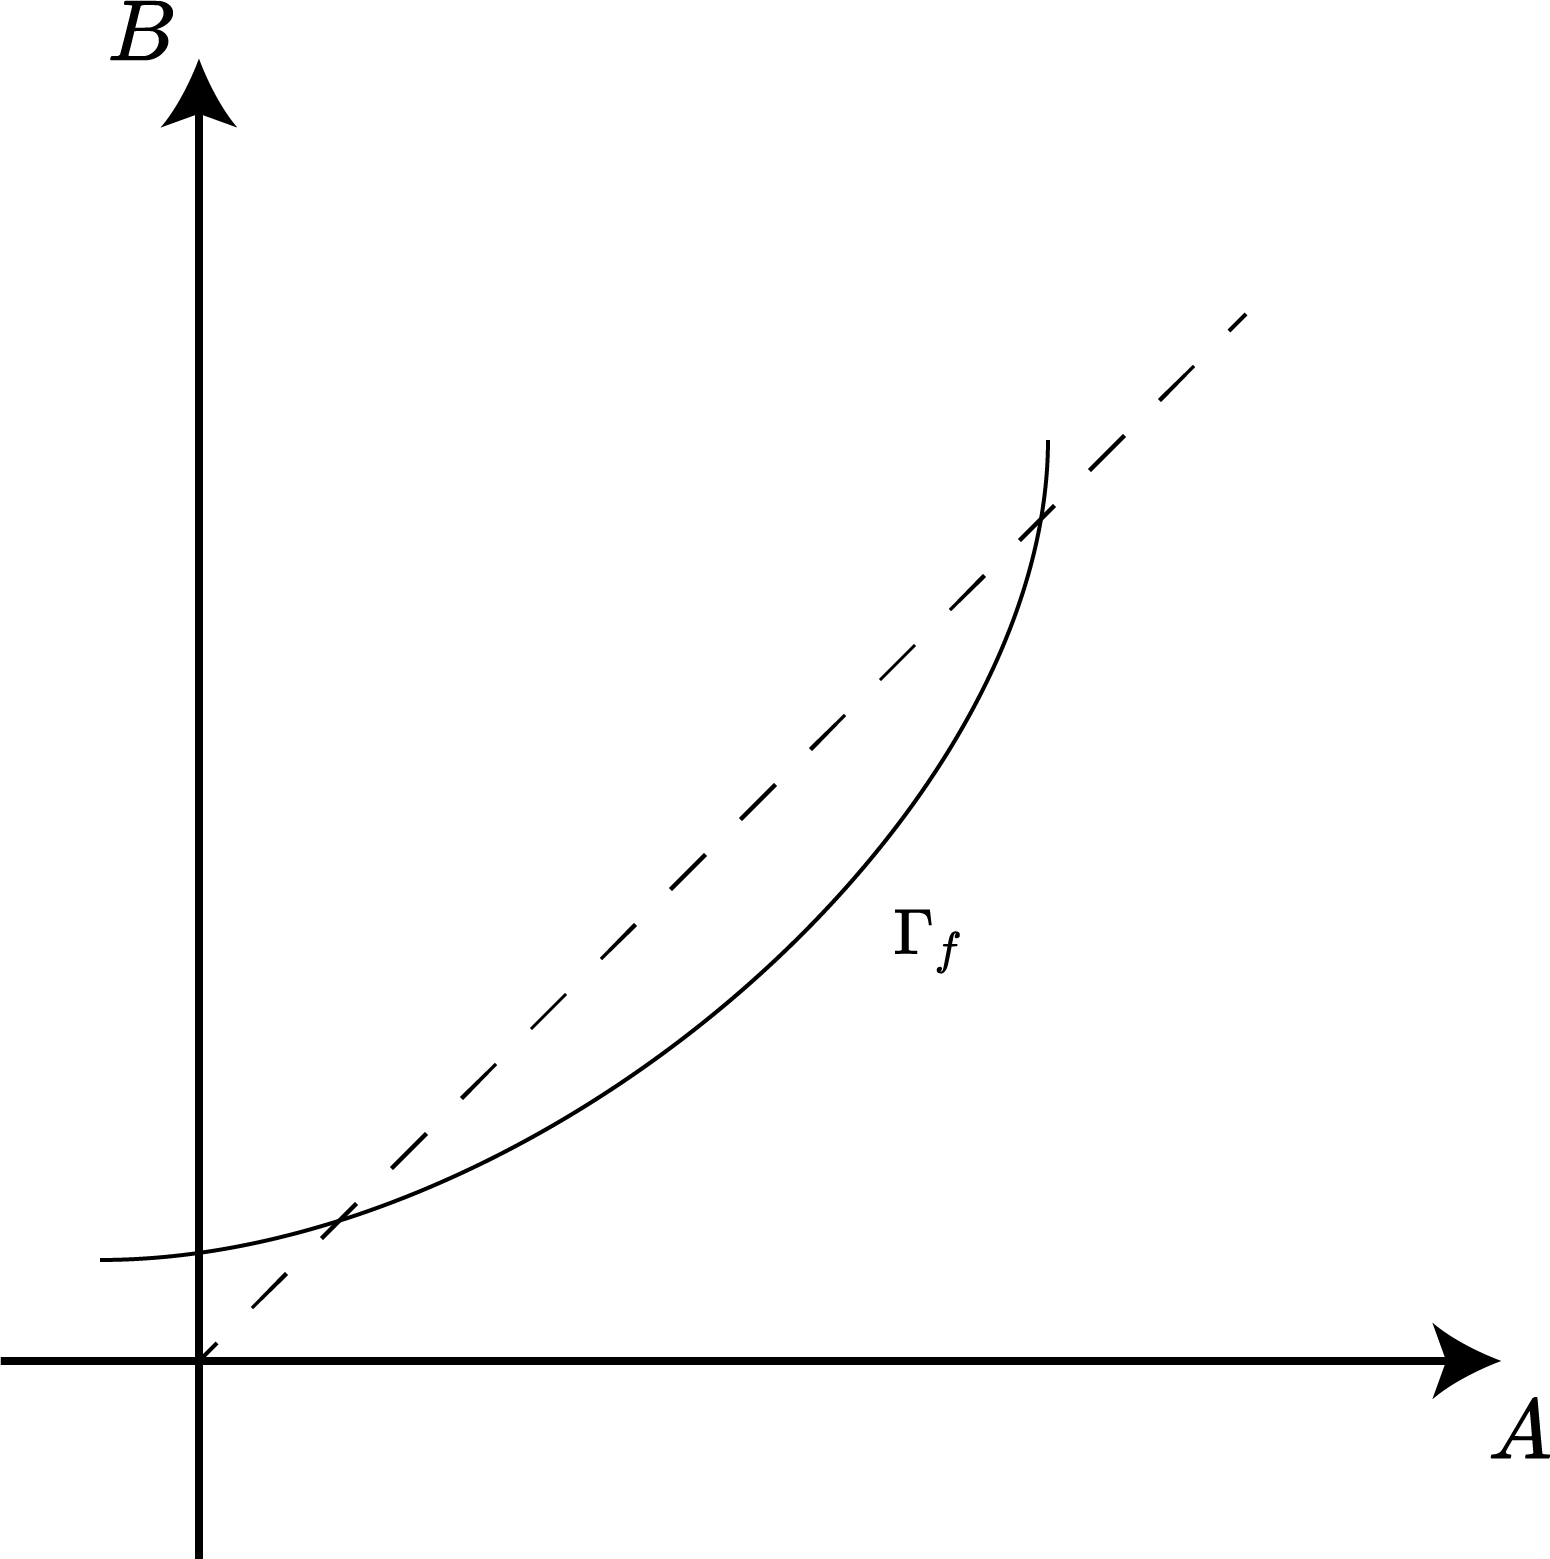
\includegraphics[width=0.3\textwidth]{images/img08.png} \quad
	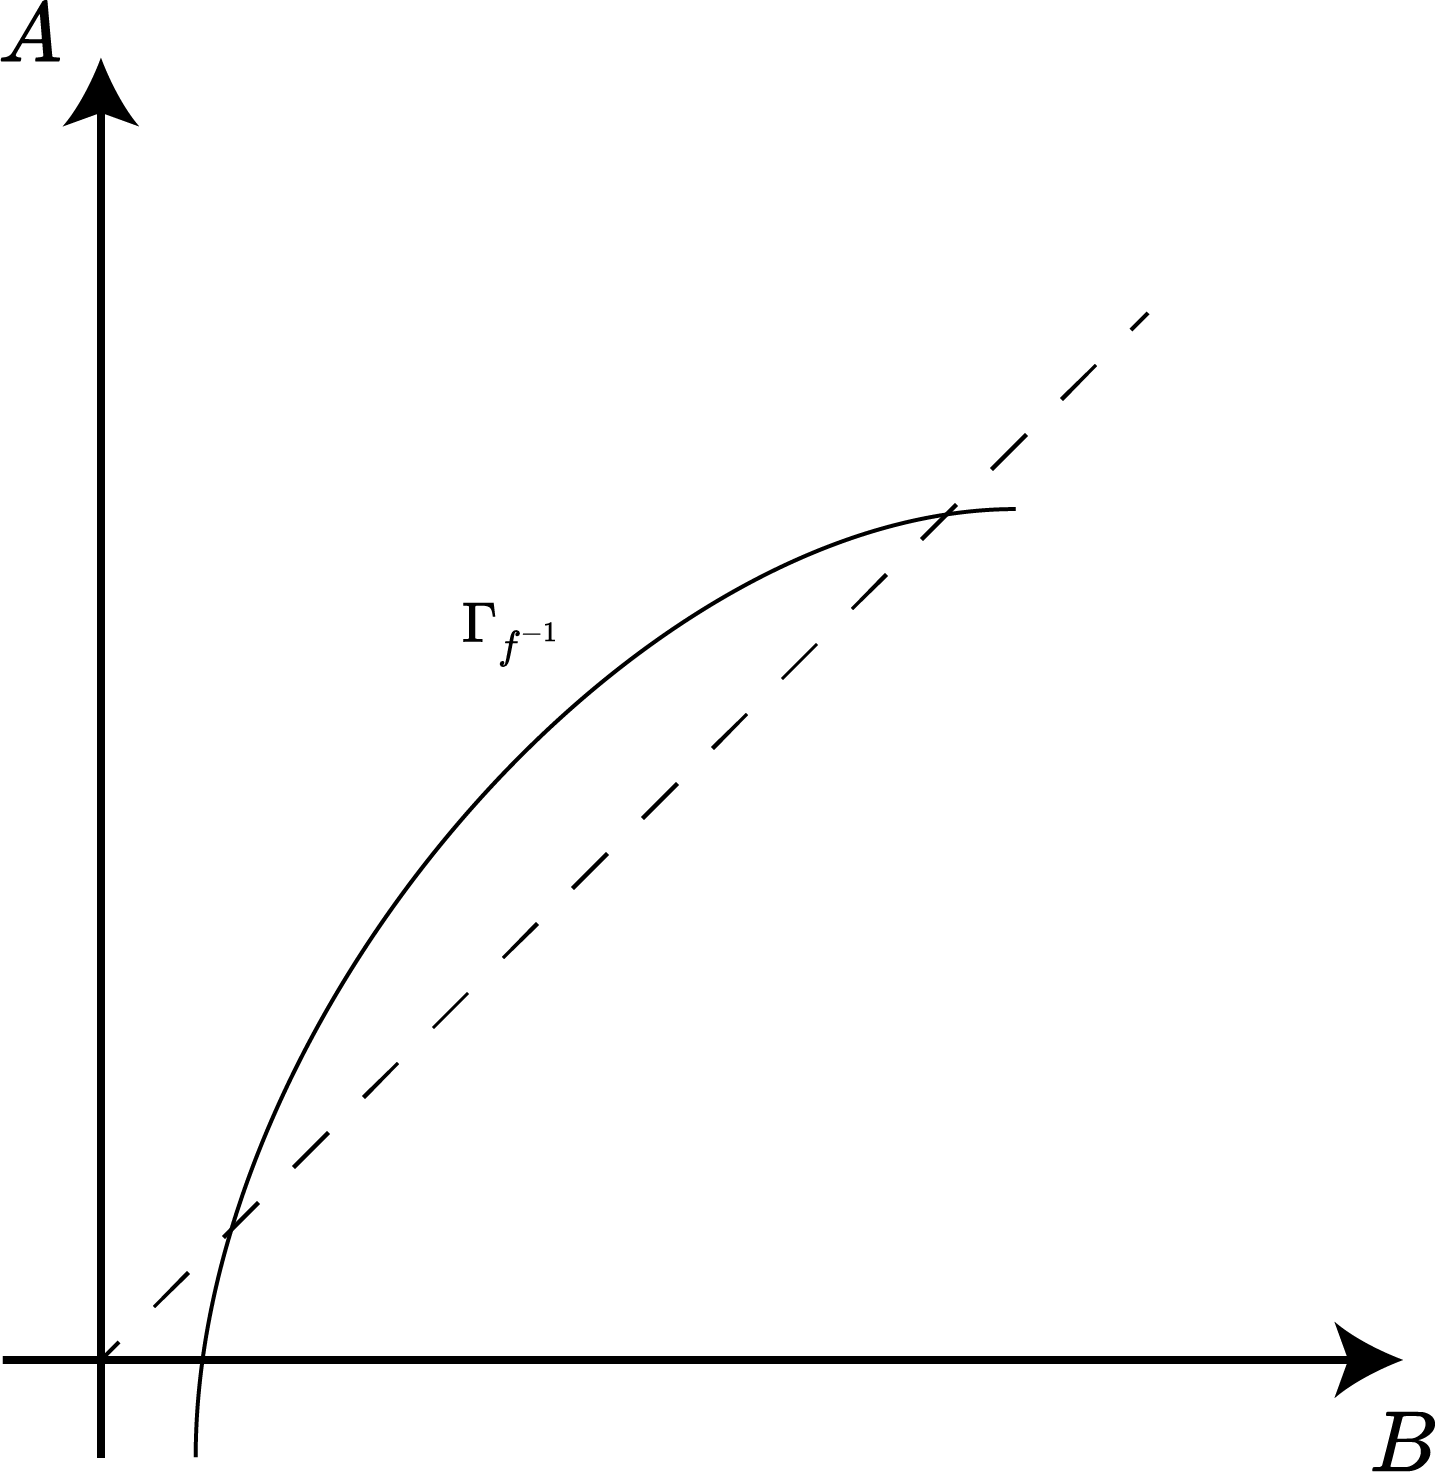
\includegraphics[width=0.3\textwidth]{images/img09.png}\\
	$\Gamma_{f^{-1}} = $ Spiegeln von $\Gamma_f$ an Winkelhalbierenden.
\end{bsp}
\subsection{Schubfachprinzip und endliche Mengen}
Notation: Sei $n\in\mathbb{N}. [n] := \{1,\ldots,n\}$ ist gegeben durch:
$$[1] = \{1,\ldots,1\} = \{1\}$$
$$[n+1] = \{1,\ldots,n,n+1\} = [n] \cup \{n+1\}\text{ induktive Def.} n\in\mathbb{N}$$
$$[2]=\{1,2\}, [3]=\{1,2,3\}$$
\begin{satz}[Schubfachprinzip]
	Ist $f:[m]\rightarrow [n] (m,n\in\mathbb{N})$ injektiv, dann ist $m\leq n$.
\end{satz}
\begin{bew}
	Fassen obige Aussage als $A(n)$ auf, die für alle $m\in\mathbb{N}$ zu zeigen ist.\\
	Induktionsanfang: $$n=1: f:[m] \rightarrow \{1\} \text{ injektiv} \Rightarrow m=1, \text{ da sonst } f(1) = 1 = f(2) \text{\Lightning zu Injektivität}.$$
	Induktionsschritt:\\
	Induktionsvoraussetzung: $A(n)$ ist wahr für $n\in\mathbb{N}$.\\
	Zu zeigen: $A(n+1)$ ist wahr.\\
	Angenommen, $f:[m]\rightarrow[n+1] = [n] \cup \{n+1\}$ sei injektiv.\\
	Zu zeigen: $m\leq n+1$\\
	Fallunterscheidung:
	\begin{enumerate}
		\item Ang. $m=1 \Rightarrow m=1\leq n+1\checkmark$
		\item Ang. $m>1, m\in\mathbb{N} \overset{\text{Satz 3.5.8}}{\Rightarrow} m-1\in\mathbb{N}$\\
		$(*)$ Beh.: $\exists$ inj. $\tilde{f}: \{1,\ldots,m-1\}\rightarrow\{1,\ldots,n\}$.\\
		$$\overset{(*) + \text{IV}}{\Rightarrow} m-1\leq n, \text{ d.h. } m\leq n+1 \Rightarrow A(n+1) \text{ ist wahr}.$$		
	\end{enumerate}
	Beweis von $(*)$:\\
	Angenommen, $\exists f: [m]\rightarrow[n+1]$ inj.\\
	Dann $\exists \tilde{f}: [m+1]\rightarrow [m+1]\rightarrow[n]$ inj.\\
	Fallunterscheidung:
	\begin{itemize}
		\item Ang. $f(k)\in [n] \forall 1\leq k \leq m-1$. Dann setze $\tilde{f}(k) := f\vert_{[m-1]}\\
		\tilde{f}(k) := f(k), 1\leq k\leq m-1$\\
		(Nachrechnen $\tilde{f}$ ist injektiv.)
		\item $\exists j\in\mathbb{N}, 1\leq j\leq m-1$ mit $f(j) = n+1$.\\
		Dann def. $\tilde{f}: [m-1]\rightarrow [n]$
		$$\tilde{f}(k) :=
		\begin{cases}
			f(k), 1 \leq k \leq m-1, k\neq j\\
			f(m), k=j
		\end{cases}$$
		Man prüfe nach $\tilde{f}: [m-1]\rightarrow [n]$ injektiv!
	\end{itemize}
\end{bew}
\begin{kor}
	Sind $n,m\in\mathbb{N}$ und $f:[m]\rightarrow[n]$ bijektiv $\Rightarrow m=n$.
\end{kor}
\begin{bew}
	Nach Voraussetzung ist $f: [m]\rightarrow[n]$ injektiv und $f^{-1}:[n]\rightarrow[m]$ auch injektiv.\\
	$\Rightarrow m\leq n \wedge n \leq m \Rightarrow m = n$.
\end{bew}
\begin{defi}
	Eine Menge $M$ ist endlich, falls $M=\emptyset$ oder falls $n\in\mathbb{N}_0$ und eine Bijektion $f:{1,\ldots,n}\rightarrow M$ existiert.\\
	Die Anzahl der Elemente von $M$ ($\#M$) ist dann $\#M:=n$, setzen $\#\emptyset := 0$. Eine Menge ist unendlich, falls sie nicht endlich ist.
	\begin{bem}
		Ist $M$ endlich, so ist $\#M$ wohldefiniert. \\
		Angenommen: 
		$$\begin{array}{lr}
		f:[n]\rightarrow M\\
		g:[m]\rightarrow M
		\end{array}
		\text{ beide bijektiv.}$$
		$$[n]\overset{f}{\longrightarrow} M \overset{g}{\longleftarrow} [m]$$
		$h:= f^{-1}\circ g = [m]\rightarrow[n]$ ist auch bijektiv. $\overset{\text{Korr. 2}}{\Rightarrow} m=n.$
	\end{bem}
	Weiter in Definition:\\
	Zwei Mengen $A,B$ heißen gleichmächtig, falls es eine Bijektion $f: A\rightarrow B$ gibt, schreiben $A\sim B$. Eine Menge $A$ heißt abzählbar, falls $A$ endlich ist oder es eine Bijektion $f: \mathbb{N}\rightarrow A$ gibt. Ist $A$ abzählbar und unendlich, so heißt $A$ abzählbar unendlich.
\end{defi}
\begin{bem}
	Satz von Cantor und Berenstein:\\
	Ang. $\exists$ Injektion $f:A\rightarrow B, f:B\rightarrow A$, dann $\exists$ Bijektion $h:A\rightarrow B$.
\end{bem}
\begin{bew}
	Siehe Kolmogorov-Fomin: Introductory Real Analysis.\\
	Könnten definieren $A\leq B$, falls es eine inj. Funktion $f: A\rightarrow B$ gibt.\\
	$A\leq B \wedge B\leq A \Leftrightarrow A\sim B$.
\end{bew}
\begin{bem}
	$A\leq B$ heißt Kardinalität von $A$ ist kleiner gleich der Kardinalität von $B$.
	\begin{enumerate}
		\item Ist $B\subset A$ und $A$ endlich, so ist $B$ endlich und $\#B \leq \# A$.
		\item $A,B$ endlich und disjunkt, $A\cap B = \emptyset \Rightarrow \#(A\cup B) = \#A + \#B$.
	\end{enumerate}
\end{bem}
\begin{satz}
	Zwei Aussagen:
	\begin{enumerate}
		\item Jede Teilmenge einer abzählbaren Menge ist abzählbar.
		\item Sind für $j\in\N \quad A_j$ abzählbare Mengen. Dann ist $\bigcup_{j\in\N}$ abzählbar.
	\end{enumerate}
\end{satz}
\begin{bew}
	Beweis unterteilen:
	\begin{enumerate}
		\item Sei $A$ abzählbar. Ist $A$ endlich, so ist auch jedes $B\subset A$ endlich, und somit abzählbar.\\
		Sei $A$ abzählbar unendlich. Dann existiert eine Bijektion $f: \N \rightarrow A$ und setzen wir $a_n := f(n)$, so ist
		$$A = \bigcup_{n\in\N} \{a_n\} = \{a_1, a_2,\ldots\}.$$
		Ist $B\subset A$, so existieren $n_j \in\N, 1\leq n_1<n_2<\ldots$ mit $$B = \{a_{n_1}, a_{n_2}, \ldots\}.$$
		Gibt es nur endlich viele $n_j$, so ist $B$ endlich, andernfalls ist $h: \N \rightarrow B, g \mapsto h(j) := a_{n_j}$
		eine Bijektion.
		\item o.B.d.A. sind alle $A_j$ paarweise verschieden, $A_l \cap A_m \neq \emptyset$ für \(l\neq m\).
		Wenn nicht, betrachte 
		\[B_1 := A_1, \quad B_2 := A_2 \setminus A_1,\]
		\[B_3 := A_3 \setminus \{A_1 \cup A_2\}, \ldots, \quad B_{n+1} := A_{n+1} \setminus \{A_1\cup\ldots\cup A_n\}\]
		Dann sind \(B_n\) paarweise verschieden und \[\bigcup_{l\in\N} B_l = \bigcup_{l\in\N} A_l.\]
		Schreiben \(A_l\) als Liste \(A_l = \{a_{1l}, a_{2l}, \ldots\}\)\\
		Bild:\\
		\begin{tikzpicture}
			\matrix(m)[matrix of math nodes,column sep=1cm,row sep=1cm]{
				s_{11} & s_{12} & s_{13} & s_{14} & \cdots \\
				s_{21} & s_{22} & s_{23} & s_{24} & \cdots \\
				s_{31} & s_{32} & s_{33} & s_{34} & \cdots \\
				s_{41} & s_{42} & s_{43} & \cdots \\
			};
			
			\draw[->]
			(m-1-1)edge(m-1-2)
			(m-1-2)edge(m-2-1)
			(m-2-1)edge(m-3-1)
			(m-3-1)edge(m-2-2)
			(m-2-2)edge(m-1-3)
			(m-1-3)edge(m-1-4)
			(m-1-4)edge(m-2-3)
			(m-2-3)edge(m-3-2)
			(m-3-2)edge(m-4-1);
		\end{tikzpicture}
		\\Jetzt können wir das obige rechteckige Schema diagonal abzählen! Dies liefert uns eine Bijektion von \(\N\) nach \(\bigcup_l\in\N A_l\).
	\end{enumerate}
\end{bew}
\begin{bem}
	Als Übung: Man gebe explizit eine Bijektion \(f : \N \rightarrow \N \times \N\) an!
\end{bem}
\textbf{Permutationen:}
\begin{defi}
	Eine bijektive Abbildung \(\sigma : \{1,\ldots,n\} \rightarrow \{1,\ldots,n\}\) heißt Permutation.
	\[n! = \prod_{k=1}^{n}k\]
\end{defi}
\begin{satz}
	\[n\in\N, S_n = \{\sigma: \{1,\ldots,n\}\rightarrow\{1,\ldots,n\} | \sigma \text{ ist bijektiv.}\} \Rightarrow \# S_n = n!\]
\end{satz}
\begin{bew} per Induktion\\
	\(n = 1\) ist klar.
	Beobachtung: Permutation \(\sigma \in S_n\) identifizieren mit \(n\)-Tupel \( (\sigma(1), \sigma(2), \ldots, \sigma(n))\)\\
	Induktionsannahme: \(\# S_n = n!\) für ein \(n\in\N\)\\
	Die Menge \(S_{n+1}\) ist die disjunkte Vereinigung der Teilmengen 
	\[S_{n+1, k} := \{\tau \in S_{n+1} | \tau_k = n+1 \} \quad k = 1,\ldots, n+1.\]
	z.B.: \[S_{4,2} = \{ (1,4,2,3), (2,4,3,1), (3,4,1,2), (1,4,3,2), (2,4,1,3), (3,4,1,2) \}\]
	Beobachtung: Jedem \(\tau = (\sigma_1,\ldots,\sigma_n)\in S_n\) können wir die Permutation \( (\sigma_1, \ldots, \sigma_{k-1}, \underbrace{n+1}_{k\text{-te Stelle}}, \sigma_k, \ldots, \sigma_n) \in S_{n,k} \) zuordnen und diese Abbildung ist bijektiv (nachprüfen).
	\[\Rightarrow \# S_{n+1,k} = \# S_n \]
	\[ S_{n+1} = \# (\bigcup_{k=1}^{n+1} S_{n+1,k} ) = \sum_{k=1}^{n+1} \underbrace{\# S_{n+1,k}}_{=\#S_n = n!} = \sum_{k=1}^{n+1} n! = (n+1)n! = (n+1)! \]
\end{bew}
\begin{defi}[Binomialkoeffizient]
	Für \(\alpha \in\R \) und \( k\in\N \) setzen wir
	\[ \binom{\alpha}{k} := \frac{\alpha(\alpha-1)\cdot\ldots\cdot(\alpha-k+1)}{k!}, \text{ sowie } \binom{\alpha}{0} := 1. \]
\end{defi}
\begin{lem}[Rekursionsformel für Binomialkoeffizienten]
	Für \( \alpha\in\R, k\in\N \) gilt \[ \binom{\alpha + 1}{k} = \binom{\alpha}{k} + \binom{\alpha}{k-1}. \]
\end{lem}
\begin{bew}
	Für \(k=1\) ist dies einfach zu sehen. Für \(k\geq 2\) gilt 
	\begin{align*}
		&\binom{\alpha}{k} + \binom{\alpha}{k-1} \\
		&= \frac{\alpha (\alpha-1)\cdot\ldots\cdot(\alpha-k+1)}{1\cdot2\cdot\ldots\cdot k} + \frac{\alpha (\alpha-1)\cdot\ldots\cdot(\alpha-k+2)}{1\cdot2\cdot\ldots\cdot (k-1)}\\
		&= \frac{\alpha (\alpha-1)\cdot\ldots\cdot(\alpha-k+2)(\alpha-k+1+k)}{1\cdot2\cdot\ldots\cdot k}\\
		&= \frac{(\alpha + 1)\alpha (\alpha-1)\cdot\ldots\cdot((\alpha-1)-k+1)}{1\cdot2\cdot\ldots\cdot k} = \binom{\alpha + 1}{k}
	\end{align*}
\end{bew}
\begin{bem}
	\begin{enumerate}
		Pascal Dreieck:\\
		\item Ist \(\alpha = n\in\N_0\), so können wir \(\binom{n}{k}\) ausrechnen mit dem Dreiecksschema von Blaise Pascal (1623-1662).\\
		\begin{tabular}{>{$n=}l<{$\hspace{12pt}}*{13}{c}}
			0 &&&&&&&1&&&&&&\\
			1 &&&&&&1&&1&&&&&\\
			2 &&&&&1&&2&&1&&&&\\
			3 &&&&1&&3&&3&&1&&&\\
			4 &&&1&&4&&6&&4&&1&&\\
			5 &&1&&5&&10&&10&&5&&1&\\
			6 &1&&6&&15&&20&&15&&6&&1
		\end{tabular}
		\item Ist \( \alpha=n\in\N_0 \), so folgt durch Erweitern mit \((n-k)!\) für \(n \in\N_0, k\in\{0,1,\ldots,n\} \) \[ \binom{n}{k} = \frac{n!}{k!(n-k)!} = \binom{n}{n-k}. \]
	\end{enumerate}
\end{bem}
\begin{satz} 
	Zahl der Kombinationen:\\	
	Sei \( n\in\N_0, k\in\{1,\ldots,n\} \). Dann ist die Anzahl der \(k\)-elementigen Teilmengen von \( \{1,\ldots,n\} \) gleich \( \binom{n}{k} \).
\end{satz}
\begin{bew}
	Die Behauptung gilt für \(k=0\) und beliebiges \(n\in\N\), da die leere Menge die einzige Teilmenge von \( \{1,\ldots,n\} \) mit 0 Elementen ist und nach Def. ist \( \binom{n}{0} = 1 \).\\
	Insbesondere gilt die Behauptung dann für \(n=0\).\\
	Induktiv über \(n\), wobei Behauptung für alle \(k\in\{0,1,\ldots,n\}\) zu zeigen ist.\\
	Induktionsschluss: Bestimme die Anzahl der \(k\)-elementigen Teilmengen von \(\{ 1,\ldots,n+1 \}\) (wobei wir \(k\geq 1\) annehmen können).\\
	Sei \(A\subset \{1,\ldots,n+1\}\) mit \(\#A = k\geq 1\). \\
	Diese fallen in 2 Klassen:
	Klasse 1: \(n+1 \notin A\).\\
	Klasse 2: \(n+1 \in A\).\\
	Die Mengen der Klasse 1 bestehen genau aus den \(k\)-elementigen Teilmengen von \(\{1,\ldots,n\}\).\\
	Die Mengen der 2. Klasse erhält man aus den \((k-1)\)-elementigen Teilmengen von \(\{1,\ldots,n\}\) durch Vereinigung mit \(\{n+1\}\).\\
	Also ist nach Induktionsannahme
	\begin{align*}
		&\#\{k\text{-elementige Teilmengen von } \{1,\ldots,n+1\} \}\\
		&=\#\{k\text{-elementige Teilmengen von } \{1,\ldots,n\} \} \\&+ \#\{(k-1)\text{-elementige Teilmengen von } \{1,\ldots,n\} \} \\
		&\overset{\text{IV}}{=} \binom{n}{k} + \binom{n}{k-1} \overset{\text{Lem. 8}}{=} \binom{n+1}{k}.
	\end{align*}
\end{bew}
\begin{satz}[Binomische Formel]
	\[ a,b\in\R,n\in\N:(a+b)^n = \sum_{k=0}^{n} \binom{n}{k} a^k b^{n-k}. \]
\end{satz}
\begin{bem}
	\begin{align}
		(a+b)^1 &= a+b\\
		(a+b)^2 &= a^2 + 2ab + b^2\\
		(a+b)^3 &= a^3 +3a^2b + 3ab^2 +b^3
	\end{align}
\end{bem}
\begin{bew} Induktion
	\[n=1: (a+b)^1 = a+b = \sum_{k=0}^{1}\binom{1}{k} a^kb^{1-k} \checkmark \]
	Induktionsvoraussetzung: für ein beliebiges, aber festes \(n \in\N\) gilt: 
	\[(a+b)^n = \sum_{k=0}^{n} \binom{n}{k} a^kb^{n-k}. \]
	Induktionsschritt: 
	\begin{align*}
		(a+b)^{n+1} &= (a+b) (a+b)^n = (a+b) \sum_{k=0}^{n} \binom{n}{k} a^kb^{n-k}\\
		&= \sum_{k=1}^{n+1} \binom{n}{k-1} a^kb^{n-(k-1)} + \sum_{k=0}^{n} \binom{n}{k} a^kb^{n+1-k}\\
		&= \binom{n}{n} a^{n+1} + \sum_{k=1}^{n} \binom{n}{k-1} a^kb^{n+1-k} + \sum_{k=1}^{n} \binom{n}{k} a^kb^{n+1-k} + \binom{n}{0} b^{n+1}\\
		&= \binom{n+1}{n+1} a^{n+1} + \sum_{k=1}^{n} \underbrace{\left(\binom{n}{k-1} + \binom{n}{k}\right)}_{=\binom{n+1}{k}} a^kb^{n+1-k} + \binom{n+1}{0} b^{n+1}\\
		&= \sum_{k=0}^{n+1} \binom{n+1}{k} a^kb^{n+1-k}\\
		&= \sum_{k=0}^{n+1} \binom{n+1}{k} a^kb^{n+1-k}.
	\end{align*}
\end{bew}
\textbf{Notation:} Geg. Menge \(A\), sei \[ \{0,1\}^A := \{ \text{Funktion }f:A\rightarrow \{0,1\} \} \] \(= \) Menge aller \(\{0,1\}\)-wertigen Funktionen mit Definitionsbereich \(A\).\\
Allg.: \(A,B\) Mengen, \(B^A := \{ \text{Funktion } f: a\rightarrow B\}\).
\begin{satz}
	Sei \(A\neq\emptyset\) eine endliche Menge. Dann ist \[\#(\{0,1\}^A) = 2^{\#A}.\]
\end{satz}
\begin{bew}
	Sei \(n := \# A \in\N \).\\
	\(\Rightarrow\) Bijektion \(h:\{1,\ldots,n\} \rightarrow A\).\\
	\( \Rightarrow \) können annehmen \(A = \{1,2,\ldots,n\}\)\\
	z.z. \(\#( \{0,1\}^[n] ) = 2^n\).\\
	Induktion: \(n=1 \exists \) Fkt. \(f_1,f_2 : \{1\} \rightarrow \{0,1\} \\
	f_1(1) = 0 \quad f_2(1) = 1 \)\\
	Formel stimmt für \(n=1\).
	Ang. Formel stimmt für \(n\geq 1\). Fkt. \(f: \{1,\ldots, n+1\} \rightarrow \{0,1\} \)\\
	2 Klassen: 
	\begin{enumerate}
		\item \(S_0 = \{f: \{1,\ldots,n\} \rightarrow \{0,1\}: f(n+1) = 0 \}\)
		\item \(S_1 = \{f: \{1,\ldots,n\} \rightarrow \{0,1\}: f(n+1) = 1 \}\)
	\end{enumerate}
	\[S_0 \cap S_1 = \emptyset, \{0,1\}^{[n+1]} = S_0 \cup S_1 \]
	\[\underbrace{\# S_0}_{=\#S_1} = \# (\{0,1\}^{[n]})  \overset{\text{IA}}{=} 2^n \]
	\[ \Rightarrow \# (\{0,1\}^{n+1}) = \#S_0+\#S_1 = 2^n + 2^n = 2^{n+1}. \]
\end{bew}
\begin{kor}
	Sei \(A\) endliche Menge. \\
	\(\mathcal{P}(A) = \) Potenzmenge = \(\{B | B \subseteq A\}\)\\
	\(\Rightarrow \#\mathcal{P}(A = 2^{\#A}) \).
\end{kor}
\begin{bew}
	Sei \(A\neq \emptyset \Rightarrow\mathcal{P}(\emptyset) = \{\emptyset\}, \quad 2^0 = 1 \checkmark \)\\
	Sei \(\#A \in\N\). Nach Satz 11 reicht eine Bijektion \( \varphi : \mathcal{P} \rightarrow \underbrace{\{0,1\}^A}_{= \{f: A \rightarrow \{0,1 \} \}} \). Dies wird in Lemma 13 für bel. Mengen \(A\) gemacht.
\end{bew}
\begin{lem}
	Sei \(A\neq\emptyset\). Dann sind \( \mathcal{P}(A) \) und \(\{0,1\}^A\) gleichmächtig.
\end{lem}
\begin{bew}
	Brauchen \(\varphi : \mathcal{P}(A) \rightarrow \{0,1\}^A \).\\
	Sei \(B \subseteq A \), Indikatorfunktion \[ \mathds{1}_B(x) := \begin{cases} 
	1, &x\in B\\
	0, &x\in A\setminus B
	\end{cases}
	, \mathds{1}_B : A \rightarrow \{0,1\}. \]
	Beachte: \(B = \{x\in A | \mathds{1}_B(x) = 1 \} \).\\
	Definiere \( \varphi : \mathcal{P}(A) \rightarrow \{0,1\}^A, B \mapsto \mathds{1}_B \).\\
	Beh.: \(\varphi\) ist bijektiv.
	\begin{enumerate}
		\item \( \varphi \) ist surjektiv.\\
		Sei \(f: A\rightarrow \{0,1\}\)
		\[ B_f := f^{-1} (\{1\}) = \{a \in A| f(a) = 1 \} \Rightarrow \varphi(B_f) = \mathds{1}_{B_f} = f\text{ (nachrechnen)}.\]
		\item \( \varphi \) ist injektiv.\\
		Seien \( B_1,B_2\subseteq A, B_1 \neq B_2 \).
		\begin{align*}
			B_1\setminus B_2 \neq \emptyset \vee B_2\setminus B_1 \neq \emptyset\\
			\text{o.B.d.A. } B_1 \setminus B_2 \neq \emptyset \Rightarrow \exists x \in B_2 \setminus B_1 \subset A\\
			\mathds{1}_{B_1}(x) = 0 \neq 1 = \mathds{1}_{B_2}(x)\\
			\Rightarrow \varphi(B_1) = \mathds{1}_{B_1} \neq \mathds{1}_{B_2} = \varphi(B_2).
		\end{align*}
	\end{enumerate}
\end{bew}
\begin{lem}
	Sei \(A\) Menge. Dann gibt es keine surj. Fkt. \(f: A\rightarrow \mathcal{P}(A) \).
\end{lem}
\begin{bem}
	Ist \(A\) endlich \( \Rightarrow \# \mathcal{P} (A) = 2^{\# A} > \#A \).\\
	\( \varphi: \mathcal{P}(A) \rightarrow \{0,1\}^A, \quad A\supset B \mapsto \mathds{1}_B \).
\end{bem}
\begin{bew}
	Sei \(f: A \rightarrow \mathcal{P}(A) \)
	\[ f(A) \subset A \quad \forall a \in A. \]
	Definiere \(R := \{a\in A, a \neq f(a)\} \subset A \).\\
	Angenommen \(f: A \rightarrow \mathcal{P}(A) \) ist surjektiv.
	\[ \Rightarrow \forall b\in A \exists b : B=f(b) \Rightarrow \exists a\in A : R = f(a). \]
	\(\Rightarrow\) 2 Möglichkeiten:
	\begin{enumerate}
		\item \(a\in R\) \[ a\in f(a = R = \{x\in A| x\notin f(x)\}) \text{\Lightning} \]
		\item \(a \notin R = f(a) \Rightarrow a \notin f(a) \Rightarrow a\in R \) \Lightning\\
		\( f\) kann nicht surjektiv sein!
	\end{enumerate}
\end{bew}